% Author: Alfredo Sánchez Alberca (asalber@ceu.es)
\section{Analytic geometry}

%---------------------------------------------------------------------slide----
\begin{frame}
\frametitle{Analytic geometry}
\setlength{\parskip}{0.3em}
\tableofcontents[sectionstyle=show/hide,hideothersubsections]
\end{frame}

\subsection{Vectors}

%---------------------------------------------------------------------slide----
\begin{frame}
\frametitle{Scalars}
Some phenomena of Nature can be described by a number and a unit of measurement. 

\begin{definition}[Scalar]
A \emph{scalar} is a number that expresses a magnitude without direction.
\end{definition}
\structure{\bfseries Examples} The height or weight of a person, the temperature of a gas or the time it takes a vehicle to travel a distance.

However, there are other phenomena that cannot be described adequately by an scalar. 
If, for instance, a sailor wants to head for seaport and only knows the intensity of wind, he won't know what direction to take. The description of wind requires two elements: intensity and direction. 
\end{frame}


%---------------------------------------------------------------------slide----
\begin{frame}
\frametitle{Vectors}
\begin{definition}[Vector]
A \emph{vector} is a number that expresses a magnitude and has associated an orientation and a sense.
\end{definition}

\structure{\bfseries Examples} The velocity of a vehicle or the force applied to an object. 

Geometrically, a vector is represented by an directed line segment, that is, an arrow. 
\begin{center}
\tikzsetnextfilename{analytic_geometry/vector}
% Author: Alfredo Sánchez Alberca (asalber@ceu.es)
\begin{tikzpicture}
\draw [->, color1] (0,0) node[anchor=south east]  {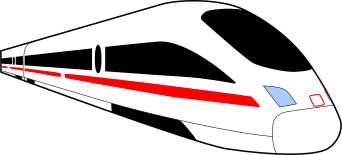
\includegraphics[scale=0.4]{img/analytic_geometry/train}} -- (2,-0.5) node[black, above, midway] {$\vec{v}$} node[sloped, pos=1, anchor=west] {direction};
\draw [decorate, decoration={brace, amplitude=5pt, mirror}, xshift=-2pt, yshift=-2pt] (0,0) -- (2,-0.5) node [midway, below, sloped, xshift=-2pt, yshift=-2pt] {magnitude};
\end{tikzpicture}

\end{center}
\end{frame}


% ---------------------------------------------------------------------slide----
\begin{frame}
\frametitle{Vector representation}
An oriented segment can be located in different places in a Cartesian space.  
However, regardless of where it is located, if the length and the direction of the segment doesn't change, the segment represents always the same vector. 

This allows to represent all vector with the same origin, the origin of the Cartesian coordinate system.
Thus, a vector can be represented by the Cartesian \emph{coordinates} of its final end in any Euclidean space.

\begin{center}
\tikzsetnextfilename{analytic_geometry/vector_coordinates}
\input{img/analytic_geometry/vector_coordinates}
\end{center}
\end{frame}


% ---------------------------------------------------------------------slide----
\begin{frame}
\frametitle{Vector from two points}
Given two points $P$ and $Q$ of a Cartesian space, the vector that starts at $P$ and ends at $Q$ has coordinates 
$\vec{PQ}=Q-P$.

\structure{\bfseries Example} Given the points $P=(2,1)$ and $Q=(3,4)$ in the real plane $\mathbb{R}^2$, the coordinates of the vector that start at $P$ and ends at $Q$ are
\[
\vec{PQ} = Q-P = (3,4)-(2,1) = (3-2,4-1) = (1,3).
\]
\begin{center}
\tikzsetnextfilename{analytic_geometry/vector_from_two_points}
% Author: Alfredo Sánchez Alberca (asalber@ceu.es)
\begin{tikzpicture}[trim axis left, trim axis right]
  \begin{axis}[
    2dfun, 
    xmin=-4, xmax=4,
    ymin=-4, ymax=4,  
    equal axis=true,
    height=4cm,
    ]
    \coordinate (0) at (0,0);
    \coordinate (P) at (2,1);
    \coordinate (Q) at (3,4);
    \draw[->, color1] (O) -- (A) node[midway, below, anchor=west] {$\vec{PQ}=(1,3)$} ;
    \draw[gray, dotted] (P) -- (P|-O);
    \draw[gray, dotted] (P) -- (P-|O);
    \draw[gray, dotted] (Q) -- (Q|-O);
    \draw[gray, dotted] (Q) -- (Q-|O);
  \end{axis}
\end{tikzpicture}

\end{center}
\end{frame}

% 
% % ---------------------------------------------------------------------slide----
% \begin{frame}
% \frametitle{Módulo de un vector}
% \begin{definition}[Módulo de un vector]
% Dado un vector $\mathbf{v}=(v_1,\cdots,v_n)$ de $\mathbb{R}^n$, se define el \emph{módulo} de $\mathbf{v}$ como
% \[
% |\mathbf{v}| = \sqrt{v_1^2+ \cdots + v_n^2}.
% \]
% \end{definition}
% El módulo de un vector coincide con la longitud del segmento que representa al vector.
% 
% \structure{\bfseries Ejemplos} 
% Sea $\mathbf{u}=(3,4)$ un vector en $\mathbb{R}^2$, entonces
% \[
% |\mathbf{u}| = \sqrt{3^2+4^2} = \sqrt{25} = 5
% \]
% Sea $\mathbf{v}=(4,7,4)$ un vector en $\mathbb{R}^3$, entonces
% \[
% |\mathbf{v}| = \sqrt{4^2+7^2+4^2} = \sqrt{81} = 9
% \]
% \end{frame} 
% 
% 
% % ---------------------------------------------------------------------slide----
% \begin{frame}
% \frametitle{Vectores unitarios}
% \begin{definition}[Vector unitario]
% Se dice que un vector $\mathbf{v}$ de $\mathbb{R}^n$ es \emph{unitario} si su módulo es 1, es decir $|\mathbf{v}|=1$.
% \end{definition}
% Especial atención merecen los vectores unitarios que siguen la dirección de los ejes de coordenadas, estos vectores se llaman \emph{vectores coordenados}.
% \begin{columns}
% \begin{column}{.48\textwidth}
% En $\mathbb{R}^2$ los vectores coordenados son 
% \[
% \mathbf{i}=(1,0)\mbox{ y }\mathbf{j}=(0,1)
% \]
% \begin{center}
% \scalebox{1}{\input{img/geometria_analitica/vectores_unitarios_r2}}
% \end{center}
% \end{column}
% \begin{column}{.48\textwidth}
% En $\mathbb{R}^3$ los vectores coordenados son 
% \[
% \mathbf{i}=(1,0,0)\mbox{, }\mathbf{j}=(0,1,0) \mbox{ y } \mathbf{k}=(0,0,1)
% \]
% \begin{center}
% \scalebox{1}{\input{img/geometria_analitica/vectores_unitarios_r3}}
% \end{center}
% \end{column}   
% \end{columns}
% \end{frame} 
% 
% 
% % ---------------------------------------------------------------------slide----
% \begin{frame}
% \frametitle{Suma de vectores}
% \begin{definition}[Suma de vectores]
% Dados dos vectores $\mathbf{u}=(u_1,\cdots,u_n)$ y $\mathbf{v}=(v_1,\cdots,v_n)$ de $\mathbb{R}^n$, se define la
% \emph{suma} de $\mathbf{u}$ y $\mathbf{v}$ como
% \[
% \mathbf{u}+\mathbf{v} = (u_1+v_1,\ldots, u_n+v_n).
% \]
% \end{definition}
% 
% \structure{\bfseries Ejemplo} 
% Sean $\mathbf{u}=(3,1)$ y $\mathbf{v}=(2,3)$ dos vectores en $\mathbb{R}^2$, entonces
% \[
% \mathbf{u}+\mathbf{v} = (3+2,1+3) = (5,4).
% \]
% 
% \begin{center}
% \scalebox{0.8}{\input{img/geometria_analitica/suma_vectores}}
% \end{center}
% \end{frame} 
% 
% 
% %---------------------------------------------------------------------slide----
% \begin{frame}
% \frametitle{Producto de un vector por un escalar}
% \begin{definition}[Producto de un vector por un escalar]
% Dado un vector $\mathbf{v}=(v_1,\cdots,v_n)$ de $\mathbb{R}^n$, y un escalar $a\in \mathbb{R}$, se define el
% \emph{producto} de $a$ por $\mathbf{v}$ como
% \[
% a\mathbf{v} = (av_1,\ldots, av_n).
% \]
% \end{definition}
% \structure{\bfseries Ejemplo}
% Sean el vector $\mathbf{v}=(2,1)$ en $\mathbb{R}^2$ y el escalar $a=2$, entonces
% \[
% a\mathbf{v} = 2(2,1) = (4,2).
% \]
% 
% \begin{center}
% \scalebox{0.8}{\input{img/geometria_analitica/producto_por_escalar}}
% \end{center}
% \end{frame}  
% 
% 
% %---------------------------------------------------------------------slide----
% \begin{frame}
% \frametitle{Expresión de un vector como combinación lineal de los vectores coordenados}
% La suma de vectores y el producto de un vector por un escalar permite expresar cualquier vector como una combinación lineal de los vectores coordenados.
% 
% En el caso del espacio real $\mathbb{R}^3$, cualquier vector $\mathbf{v}=(v_1,v_2,v_3)$ puede expresarse como   
% \[
% \mathbf{v}=(v_1,v_2,v_3) = v_1\mathbf{i}+v_2\mathbf{j}+v_3\mathbf{k}.
% \]
% 
% \begin{center}
% \scalebox{0.8}{\input{img/geometria_analitica/combinacion_lineal_vectores_coordenados}}
% \end{center}
% \end{frame} 
% 
% 
% %---------------------------------------------------------------------slide----
% \begin{frame}
% \frametitle{Producto escalar}
% \begin{definition}[Producto escalar]
% Dados dos vectores $\mathbf{u}=(u_1,\cdots,u_n)$ y $\mathbf{v}=(v_1,\cdots,v_n)$ de $\mathbb{R}^n$, se define el
% \emph{producto escalar} de $\mathbf{u}$ y $\mathbf{v}$ como
% \[
% \mathbf{u}\cdot \mathbf{v} = u_1v_1 + \cdots + u_nv_n.
% \]
% \end{definition}
% \structure{\bfseries Ejemplo} 
% Sean $\mathbf{u}=(3,1)$ y $\mathbf{v}=(2,3)$ dos vectores en $\mathbb{R}^2$, entonces
% \[
% \mathbf{u}\cdot\mathbf{v} = 3\cdot 2 +1\cdot 3 = 9.
% \]
% 
% Se cumple que
% \[
% \mathbf{u}\cdot\mathbf{v} =  |\mathbf{u}||\mathbf{v}|\cos\alpha
% \]
% donde $\alpha$ es el ángulo que forman los vectores.
% \end{frame} 
% 
% 
% %---------------------------------------------------------------------slide----
% \begin{frame}
% \frametitle{Vectores paralelos}
% \begin{definition}[Vectores paralelos]
% Dos vectores $\mathbf{u}$ y $\mathbf{v}$ son \emph{paralelos} si existe un valor $a\in\mathbb{R}$ tal que
% \[
% \mathbf{u} = a\mathbf{v}.
% \]
% \end{definition}
% 
% \structure{\bfseries Ejemplos} 
% Los vectores $\mathbf{u}=(-4,2)$ y $\mathbf{v}=(2,-1)$ en $\mathbb{R}^2$ son paralelos, ya que
% \[
% \mathbf{v}= (-4,2) = -2(2,-1) = -2\mathbf{v}.
% \]
% 
% \end{frame} 
% 
% 
% %---------------------------------------------------------------------slide----
% \begin{frame}
% \frametitle{Vectores ortogonales y ortonormales}
% \begin{definition}[Vectores ortogonales y ortonormales]
% Dos vectores $\mathbf{u}$ y $\mathbf{v}$ son \emph{ortogonales} si su producto escalar es nulo
% \[
% \mathbf{u}\cdot \mathbf{v} = 0.
% \]
% Si además el módulo de ambos vectores es la unidad $|\mathbf{u}|=|\mathbf{v}|=1$, entonces se dice que son \emph{ortonormales}.
% \end{definition}
% 
% Los vectores ortogonales son perpendiculares entre sí, es decir, forman un ángulo de $90^\circ$.
% 
% \structure{\bfseries Ejemplos} 
% Los vectores $\mathbf{u}=(2,1)$ y $\mathbf{v}=(-2,4)$ en $\mathbb{R}^2$ son ortogonales, ya que
% \[
% \mathbf{u}\mathbf{v} = 2\cdot -2 +1\cdot 4 = 0,
% \]
% pero no son ortonormales ya que $|\mathbf{u}| = \sqrt{2^2+1^2} \neq 1$ y  $|\mathbf{v}| = \sqrt{-2^2+4^2} \neq 1$.
% 
% Los vectores $\mathbf{i}=(1,0)$ y $\mathbf{j}=(0,1)$ en $\mathbb{R}^2$ son ortonormales, ya que
% \[
% \mathbf{i}\mathbf{j} = 1\cdot 0 +0\cdot 1 = 0, \quad |\mathbf{i}| = \sqrt{1^2+0^2} = 1,  \quad |\mathbf j| = \sqrt{0^2+1^2} = 1.
% \]
% \end{frame}  
% 
% 
% 
% \subsection{Rectas}
% %---------------------------------------------------------------------slide----
% \begin{frame}
% \frametitle{Ecuación vectorial de la recta}
% \begin{definition}[Ecuación vectorial de la recta]
% Sea $l$ una recta del espacio $\mathbb{R}^n$ y sean $P=(p_1,\ldots,p_n)$ un punto cualquiera de la recta y
% $\mathbf{v}=(v_1,\ldots,v_n)$ un vector cualquiera con la misma dirección que la recta.
% La ecuación
% \[
% l: X= P + t\mathbf{v} = (p_1,\ldots,p_n)+t(v_1,\ldots,v_n) = (p_1+tv_1,\ldots,p_n+tv_n).
% \]
% parametriza a $l$ en función de $t\in \mathbb{R}$, y se conoce como \emph{ecuación vectorial de la recta}.
% \end{definition}
% \begin{columns}
% \begin{column}{.48\textwidth}
% \structure{\bfseries Ejemplo} 
% Considerese la recta del espacio real $\mathbb{R}^3$ que aparece en la gráfica. Un punto de la recta es $P=(1,1,2)$ y un vector director es $\mathbf{v}=(-1,2,2)$, luego su ecuación vectorial es
% \begin{align*}
% l &: X= P + t\mathbf{v} = (1,1,2)+t(-1,2,1) =\\
% &= (1-t,1+2t,2+t)\quad t\in\mathbb{R}.
% \end{align*}
% \end{column}
% \begin{column}{.48\textwidth}
% \begin{center}
% \scalebox{0.8}{\input{img/geometria_analitica/ecuacion_vectorial_recta}}
% \end{center}
% \end{column}
% \end{columns}
% \end{frame} 
% 
% 
% %---------------------------------------------------------------------slide----
% \begin{frame}
% \frametitle{Ecuaciones paramétricas y cartesianas de la recta}
% De la ecuación vectorial de una recta $l: X=P + t\mathbf{v}=(p_1+tv_1,\ldots,p_n+tv_n)$ se obtienen facilmente las coordenadas de los puntos que forman parte de la recta mediante $n$ ecuaciones paramétricas:
% \[
% x_1(t)=p_1+tv_1, \ldots, x_n(t)=p_n+tv_n
% \]
% donde, si $\mathbf{v}$ es un vector cuyas coordenadas son no nulas ($v_i\neq 0$ $\forall i$), se puede despejar el parámetro $t$ en cada una de ellas e igualarlas,
% \[
% \frac{x_1-p_1}{v_1}=\cdots = \frac{x_n-p_n}{v_n}
% \] 
% 
% \structure{\bfseries Ejemplo} 
% Dada la ecuación vectorial de la recta $l: X=(1,1,2)+t(-1,2,1) =(1-t,1+2t,2+t)$ en el espacio real $\mathbb{R^3}$, sus
% ecuaciones paramétricas son
% \[
% x(t) = 1-t, \quad y(t)=1+2t, \quad z(t)=2+t,
% \]
% y sus ecuaciones cartesianas son
% \[
% \frac{x-1}{-1}=\frac{y-1}{2}=\frac{z-2}{1}
% \]
% \end{frame} 
% 
% 
% %---------------------------------------------------------------------slide----
% \begin{frame}
% \frametitle{Ecuación punto-pendiente de una recta en el plano}
% En el caso particular del plano cartesiano $\mathbb{R^2}$, si se tiene una recta con ecuación vectorial $l: X=P+t\mathbf{v}=(x_0,y_0)+t(a,b)
% = (x_0+ta,y_0+tb)$, sus ecuaciones paramétricas son
% \[
% x(t)=x_0+ta,\quad y(t)=y_0+tb
% \]
% y sus ecuación cartesiana es
% \[
% \frac{x-x_0}{a} = \frac{y-y_0}{b}.
% \]  
% A partir de aquí, pasando $b$ multiplicando al otro lado de la ecuación, se obtiene 
% \[
% y-y_0 = \frac{b}{a}(x-x_0) \mbox{ o bien } y-y_0+m(x-x_0),
% \]
% llamando $m=b/a$. Esta ecuación se conoce como ecuación en la forma \emph{punto-pendiente}.
%  
% \end{frame} 
% 
% 
% %---------------------------------------------------------------------slide----
% \begin{frame}
% \frametitle{Pendiente de una recta en el plano}
% \begin{definition}[Pendiente de una recta]
% Dada una recta $l: X=P+t\mathbf{v}$ en el plano real $\mathbb{R}^2$, con vector director $\mathbf{v}=(a,b)$, se define la pendiente de $l$ como $b/a$.
% \end{definition}
% 
% Recordar que dados dos puntos $Q=(x_1,y_1)$ y $Q=(x_2,y_2)$ de la recta $l$, se puede tomar como vector director el vector que los une, que tiene coordenadas $\vec{PQ}=Q-P=(x_2-x_1,y_2-y_1)$, de manera que la pendiente de $l$ será 
% $\dfrac{y_2-y_1}{x_2-x_1}$, es decir, el cociente entre lo que cambia la coordenada $y$ y lo que cambia la coordenada $x$.
% 
% \begin{center}
% \scalebox{0.7}{\input{img/geometria_analitica/pendiente_recta}}
% \end{center}
% \end{frame} 
% 
% 
% 
% \subsection{Planos}
% %---------------------------------------------------------------------slide----
% \begin{frame}
% \frametitle{Ecuación del plano en el espacio real}
% Para llegar a la ecuación de un plano en el espacio real $\mathbb{R}^3$ se puede partir de un punto del plano $P=(x_0,y_0,z_0)$ y de un vector perpendicular al plano $\mathbf{v}=(a,b,c)$. 
% Entonces, para cualquier punto del plano $Q=(x,y,z)$ se cumple que el vector $\vec{PQ} = (x-x_0,y-y_0,z-z_0)$ es ortogonal a $\mathbf{v}$, por lo que su producto escalar se anulará
% \[
% \vec{PQ}\cdot\mathbf{v} = (x-x_0,y-y_0,z-z_0)(a,b,c) = a(x-x_0)+b(y-y_0)+c(z-z_0) = 0.
% \]
% 
% \begin{center}
% \scalebox{0.8}{\input{img/geometria_analitica/ecuacion_plano}}
% \end{center}
% \end{frame} 



